\subsection{Vectors and Geometry}

\subsubsection{Vectors}
Vectors arise from describing things that have both magnitude and direction (such as force or velocity). The coordinates of a vector $\vec{a}$ can be defined as $\langle a_1, a_2, a_3\rangle$. This is the expression for a vector in three dimensions but a vector can be also be defined in an arbitrary number of dimensions.\\
\\
The length of a vector can be determined using Pythagorean's theorem and is denoted by $\|\vec{a}\|$ for where $\vec{a}$ is a vector. The length is equal to,
$$\|\vec{a}\|=\sqrt{a_1^2+a_2^2+a_3^2+\cdots+a_n^2}$$
Ex: The length of $\brangle{1,2,3}$ is $\sqrt{1+4+9}=\sqrt{14}$\\
\\
A vector can be multiplied by a scalar as such:
$$k\vec{a}=\brangle{ka_1,ka_2,ka_3,\ldots,ka_n}$$
This stretches and contracts the vector. If you multiply by a negative, the vector will flip directions.\\
Ex: $2\brangle{1,1}=\brangle{2,2 }$\\
Ex2: $-1\brangle{2,1}=\brangle{-2, -1}$\\
\\
A unit vector is a vector whose magnitude is $1$ and is considered to only have a directional component (sometimes called a direction vector)
$$\hat{a}=\dir\vec{a}=\frac{\vec{a}}{\|\vec{a}\|}$$
\begin{align*}
    &\text{Ex: }\dir\brangle{2,7}=\frac{\brangle{2,7}}{\sqrt{4+49}}=\brangle{\frac{2}{\sqrt{53}},\frac{7}{\sqrt{53}}}
\end{align*}
Two vectors can be added by adding each element.
$$\vec{a}+\vec{b}=\brangle{a_1+b_1,a_2+b_2}$$
Ex: $\brangle{2,0}+\brangle{1,2}=\brangle{3,2}$
Geometrically, vector addition is the same as adding the two vectors tip to tail.\\
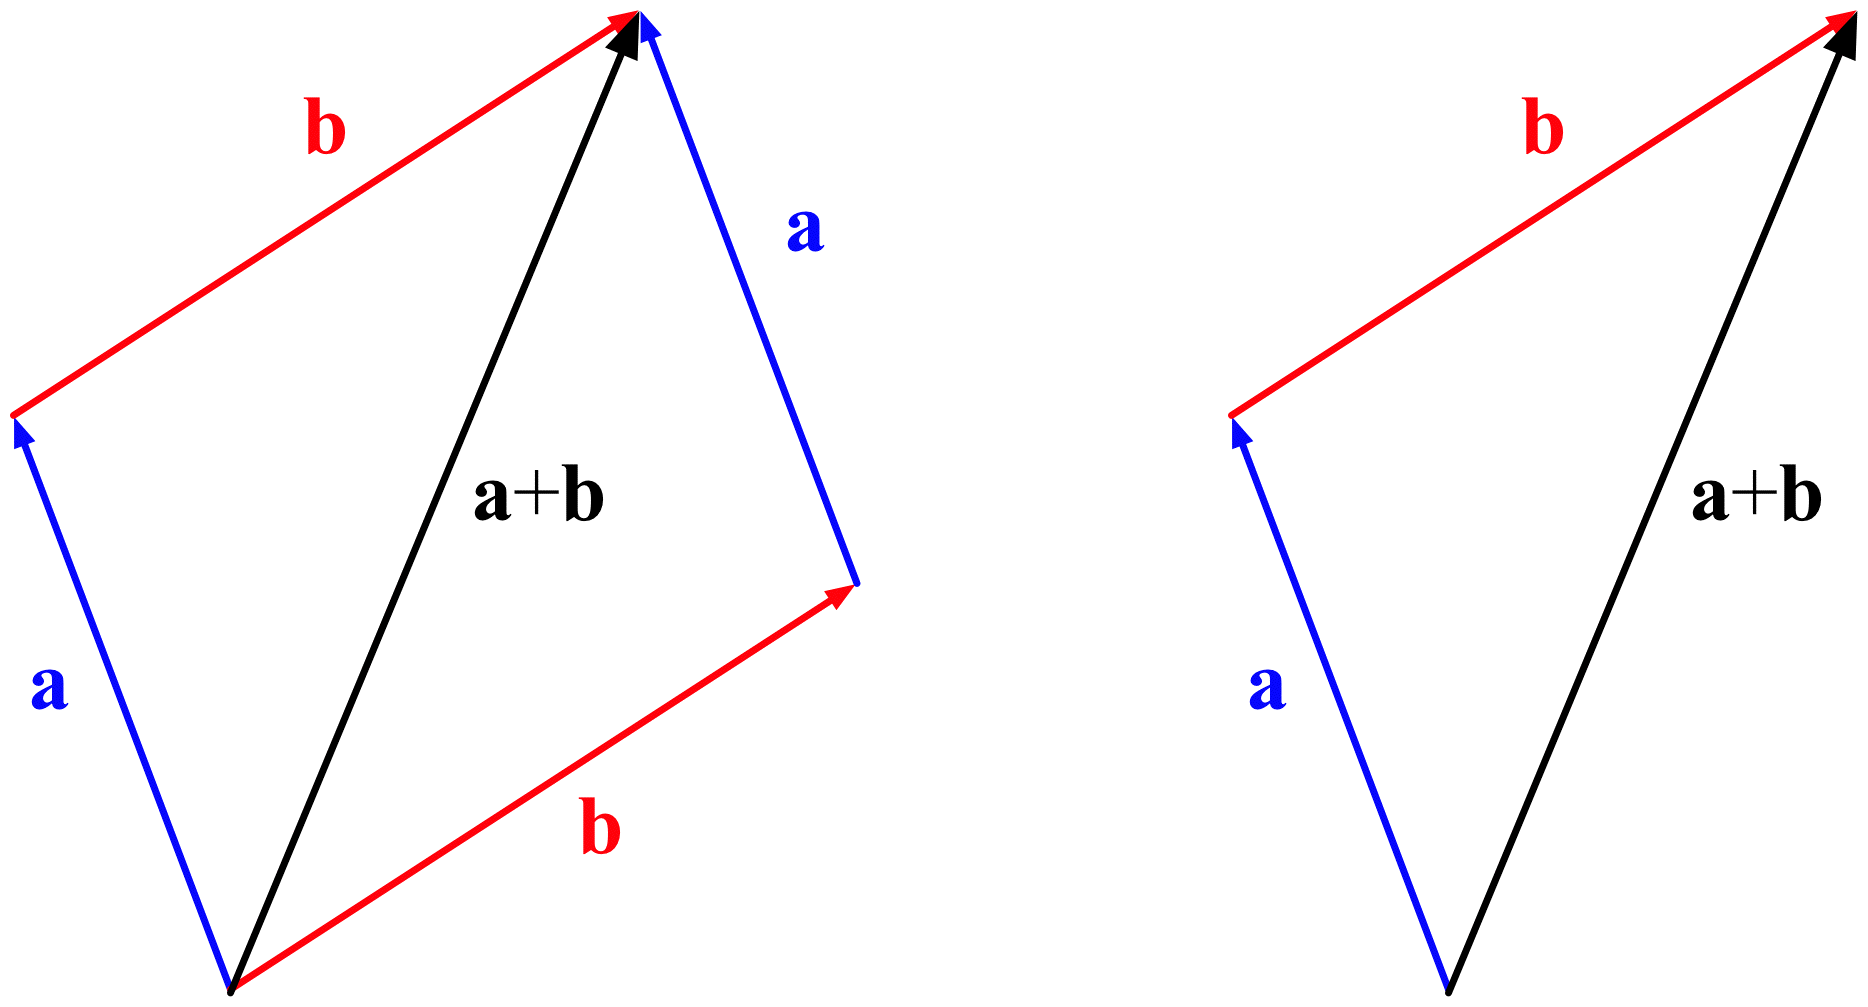
\includegraphics[scale=0.2]{Images/LinearAlgebraPictures/VectorAddition.png}\\
Similarly, vector subtraction is represented as
$$\vec{a}-\vec{b}=\brangle{a_1-b_1,\,a_2-b_2}$$
and is shown geometrically as the vector from $\vec{b}$ to $\vec{a}$\\
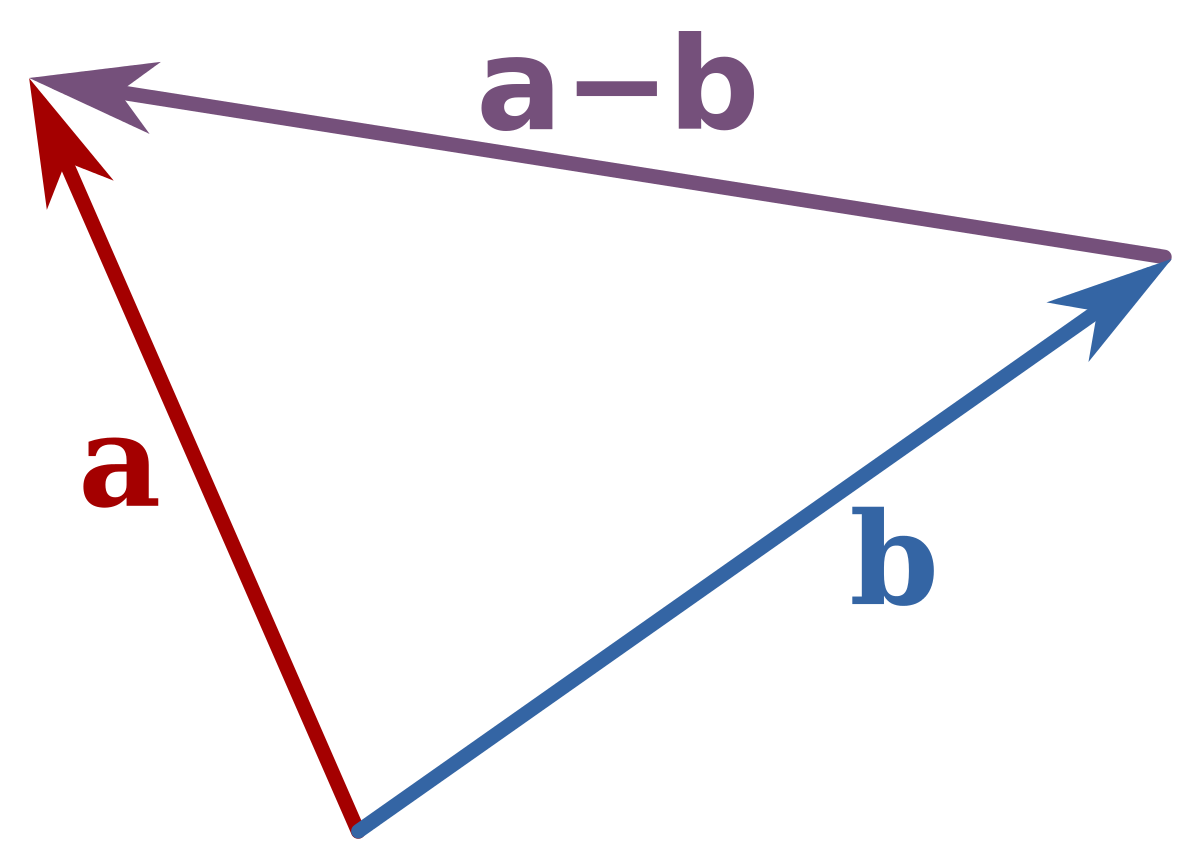
\includegraphics[scale=0.15]{Images/LinearAlgebraPictures/VectorSubtraction.png}\\
The dot product is one form of multiplication of vectors. It is defined as
$$\vec{a}\cdot\vec{b}=a_1b_1+a_2b_2$$
*Notice that the output of a dot product is a scalar.\\
Ex: $\brangle{2,3}\cdot\brangle{2,1}=2\cdot2+3\cdot1=4+3=7$
One useful identity of the dot product is 
$$\vec{a}\cdot\vec{a}=\|\vec{a}\|^2$$
Another identity is
$$\vec{a}\cdot\vec{b}=\|\vec{a}\|\|\vec{b}\|\cos\theta$$
where $\theta$ is the angle between $\vec{a}$ and $\vec{b}$
Proof:\\
\begin{align*}
    &\|\vec{a}-\vec{b}\|^2=(\vec{a}-\vec{b})\cdot(\vec{a}-\vec{b})=\vec{a}\cdot\vec{a}-\vec{a}\cdot\vec{b}-\vec{b}\cdot\vec{a}+\vec{b}\cdot\vec{b}=\|\vec{a}\|^2-2\vec{a}\cdot\vec{b}+\|\vec{b}\|^2
\end{align*}
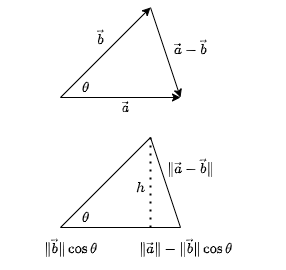
\includegraphics[scale=0.8]{Images/LinearAlgebraPictures/DotProductProof.png}
\begin{align*}
    &\|\vec{a}-\vec{b}\|^2=h^2+(\|\vec{a}\|-\|\vec{b}\|\cos\theta)^2\\
    &h=\|\vec{b}\|\sin\theta\\
    &\|\vec{a}-\vec{b}\|^2=\|\vec{b}\|^2\sin^2\theta+\|\vec{a}\|^2-2\|\vec{a}\|\|\vec{b}\|\cos\theta+\|\vec{b}\|^2\cos^2\theta\\
    &=\|\vec{a}\|^2+\|\vec{b}\|^2-2\|\vec{a}\|\|\vec{b}\|\cos\theta\\
    &\Ra\|\vec{a}\|^2-2\vec{a}\cdot\vec{b}+\|\vec{b}\|^2=\|\vec{a}\|^2+\|\vec{b}\|^2-2\|\vec{a}\|\|\vec{b}\|\cos\theta\\
    &\Ra\vec{a}\cdot\vec{b}=\|\vec{a}\|\|\vec{b}\|\cos\theta
\end{align*}
\begin{align*}
    \text{Ex: }&\text{Find the angle between $\brangle{1,2}$ and $\brangle{1,1}$}\\
    &\cos\theta=\frac{\vec{a}\cdot\vec{b}}{\|\vec{a}\|\|\vec{b}\|}=\frac{\brangle{1,2}\cdot\brangle{1,1}}{\sqrt{5}\sqrt{2}}=\frac{3}{\sqrt{10}}\\
    &\theta=\arccos\brround{\frac{3}{\sqrt{10}}}
\end{align*}
Note that if $\vec{a}\cdot\vec{b}=0$ it implies that the angle between them is $90^\circ$ and that $\vec{a}\perp\vec{b}$. In general, a vector orthogonal to $\vec{a}$ can be defined as $\vec{a}^\perp=\pm\brangle{a_2,-a_1}$\\
Proof:
\begin{align*}
    &\vec{a}\cdot\vec{b}=a_1b_1+a_2b_2=0\\
    &a_1b_1=-a_2b_2\\
    &\Ra b_1=a_2,\,b_2=-a_1\\
    &\Ra\vec{b}=\vec{a}^\perp=\pm\brangle{a_2,-a_1}
\end{align*}
Projections:\\
The projection of a vector $\vec{a}$ in the direction of $\vec{b}$ is denoted by $\proj_{\vec{b}}\vec{a}$.\\
The magnitude of the projection is $\|\vec{a}\|\cos\theta$ so we can define the projection vector as
$$\proj_{\vec{b}}\vec{a}=(\vec{a}\cdot\hat{b})\hat{b}=\frac{\vec{a}\cdot\vec{b}}{\|\vec{b}\|^2}\vec{b}$$
\begin{align*}
    \text{Ex: }&\text{Find the projection of $\brangle{2,3}$ onto $\brangle{2,1}$}\\
    &\vec{a}=\brangle{2,3},\,\vec{b}=\brangle{2,1}\\
    &\proj_{\vec{b}}\vec{a}=\frac{\brangle{2,3}\cdot\brangle{2,1}}{\|\brangle{2,1}\|^2}\brangle{2,1}=\frac{7}{5}\brangle{2,1}\\
    &=\brangle{\frac{14}{5},\frac{7}{5}}
\end{align*}
\subsubsection{Determinants and Cross Products}
The 2x2 determinant is defined as
$$\det\matrixx{a_1 & a_2\\ b_1 & b_2}=\detmatrix{a_1 & a_2\\ b_1 & b_2}=a_1b_2-a_2b_1$$
Geometrically, it represents the signed area of the parallelogram spanned by vectors $\vec{a},\,\vec{b}$.
$$A_{parallelogram}=\left|\det\matrixx{-\vec{a}-\\-\vec{b}-}\right|$$
If the determinant is equal to zero it implies the area is zero and it means that $\vec{a}$ and $\vec{b}$ are along the same line and are considered \textit{colinear}.\\
\\
Determinants in $\R^3$
$$\detmatrix{a_1 & a_2 & a_3\\b_1 & b_2 & b_3\\c_1 & c_2 & c_3}=a_1\detmatrix{b_2 & b_3\\c_2 & c_3}-a_2\detmatrix{b_1 & b_3\\c_1 & c_3}+a_3\detmatrix{b_1 & b_2\\c_1 & c_2}=a_1b_2c_3+a_2b_3c_1+a_3b_1c_2-a_1b_3c_2-a_2b_1c_3-a_3b_2c_1$$
\begin{align*}
    \text{Ex: }&\det\matrixx{1 & 2& 0\\2& 7 & 1\\ 5& 3& 3}\\
    &=1\detmatrix{7 & 1\\ 3 & 3}-2\detmatrix{ 2 &1\\ 5&3}+0\detmatrix{2 & 7\\5 & 3}\\
    &=(21-3)-2(6-5)\\
    &=16
\end{align*}
Geometrically, the 3x3 determinant represents the area of the parellelapiped spanned by $\vec{a},\,\vec{b},\,\vec{c}$
$$A_{parallelapiped}=\det\matrixx{-\vec{a}-\\-\vec{b}-\\-\vec{c}-}=\vec{a}\cdot(\vec{b}\times\vec{c})$$
Cross Product:\\
The cross product is defined as
$$\vec{a}\times\vec{b}=\brangle{a_2b_3-a_3b_2,\,a_3b_1-a_1b_3,\,a_1b_2-a_2b_1}$$
It can be more easily interpreted as
$$\vec{a}\times\vec{b}=\detmatrix{\hat{i} & \hat{j} & \hat{k}\\a_1 & a_2 & a_3\\b_1 & b_2 & b_3}$$
where $\hat{i}=\brangle{1,0,0},\,\hat{j}=\brangle{0,1,0},\,\text{and }\hat{k}=\brangle{0,0,1}$\\
The result of $\vec{a}\times\vec{b}$ will be a vector orthogonal to both $\vec{a}$ and $\vec{b}$.\\
*Note that $\vec{a}\times\vec{b}=-\vec{b}\times\vec{a}$
\begin{align*}
    \text{Ex: }&\brangle{1,1,1}\times\brangle{1,2,3}\\
    &=\detmatrix{\hat{i} & \hat{j} & \hat{k}\\1 & 1 & 1\\1&2&3}\\
    &=\hat{i}\detmatrix{1&1\\2&3}-\hat{j}\detmatrix{1&1\\1&3}+\detmatrix{1&1\\1&2}\\
    &=\brangle{1,-2,1}
\end{align*}
A useful identity is that $\|\vec{a}\times\vec{b}\|=\|\vec{a}\|\|\vec{b}\|\sin\theta$. This also happens to be the area of a parallelogram in $\R^3$.
\subsubsection{Lines and Planes}
Parametric Representation of a line:\\
The parametric form of a plane can be thought of as a scaled direction vector plus a vector from the origin to some point on the line. If we let $\vec{x}$ represent our line then we have
$$L=\brcurly{\vec{x}:\,\vec{x}=s\vec{a}+\vec{p},\,s\in\R}$$
where $\vec{a}$ is the direction vector, $s$ is a scaling variable, and $\vec{p}$ is some point on the line.\\
Ex: Find the parametric equation of a line that passes through $(1,2)$ and $(3,3)$
\begin{align*}
    &\vec{a}=(3,3)-(1,2)=\brangle{2,1}\\
    &\vec{p}=\brangle{1,2}\\
    &\Ra\vec{x}=\brangle{2,1}s+\brangle{1,2}
\end{align*}
Parametric Form of a Plane:\\
A plane is a 2D object, meaning that we will require 2 parameters ($s$ and $t$) to describe it. The parametric form for a plane is very similar to that of a line in $\R^2$, just with the addition of another scaling variable, $t$, and another direction vector $\vec{b}$.
$$P=\brcurly{\vec{x}:\,\vec{x}=s\vec{a}+t\vec{b}+\vec{p},\,s,t\in\R}$$
Ex: The points $(1,1,1)$, $(2,3,7)$, and $(0,2,0)$ lie on a plane. Write the parametric form of the plane.
\begin{align*}
    &\vec{a}=(2,3,7)-(1,1,1)=\brangle{1,2,6}\\
    &\vec{b}=(0,2,0)-(1,1,1)=\brangle{-1,1,-1}\\
    &\vec{p}=\brangle{1,1,1}\\
    &\Ra\vec{x}=s\brangle{1,2,6}+t\brangle{-1,1,-1}+\brangle{1,1,1}
\end{align*}
Equation Form of a line in $R^2$:\\
Another way to express the equation of a line is
$$n_1x_1+n_2x_2=d$$
where $n_1,\,n_2$ are components of the normal vector and $d$ is some constant that is found by plugging in a point on the line.\\
This equation is derived the following way:
\begin{align*}
    &\text{let }\vec{n}=\vec{a}^\perp\text{ and }\vec{n}\perp\vec{a}\\
    &\vec{a}\cdot\vec{n}=0\\
    &\vec{x}=\vec{a}+\vec{p}\Ra\vec{a}=\vec{x}-\vec{p}\\
    &(\vec{x}-\vec{p})\cdot\vec{n}=0\\
    &\vec{x}\cdot\vec{n}-\vec{p}\cdot\vec{n}=0\\
    &\vec{x}\cdot\vec{n}=\vec{p}\cdot\vec{n}\\
    &\text{let }\vec{p}\cdot\vec{n}=d\\
    &n_1x_1+n_2x_2=d
\end{align*}
*Note: a handy trick for calculating $\vec{n}$ in $\R^2$ is to use a similar method to the cross product:
$$\vec{n}=\pm\detmatrix{\hat{i}&\hat{j}\\a_1&a_2}$$
Ex: Write the equation of the line passing through $(1,2)$ and $(3,3)$.
\begin{align*}
    &\vec{a}=(3,3)-(1,2)=\brangle{2,1}\\
    &\vec{n}=\brangle{-1,2}\\
    &\vec{x}\cdot\vec{n}=d\\
    &-x_1+2x_2=d\\
    &\text{plug in point }(1,2):\,-1+4=d=3\\
    &-x_1+2x_2=3
\end{align*}
Ex2: Determine if the point $(5,5)$ is on the line in the example above.
\begin{align*}
    -5+2(5)=5\neq3\therefore(5,5)\text{ is not on the line.}
\end{align*}
Equation Form of a Plane in $\R^3$:\\
The equation form of a plane follows the exact same pattern but contains one more term.
$$n_1x_1+n_2x_2+n_3x_3=d$$
The only part that is slightly different is finding the normal vector $\vec{n}$. In this case, you must take the cross product of two direction vectors to find the normal (as it will be orthogonal to both and, therefore, the plane). $\vec{n}=\pm\vec{a}\times\vec{b}$\\
Ex: Find the equation form of the plane that contains $(1,1,1)$, $(2,3,7)$, and $(0,2,0)$
\begin{align*}
    &\vec{a}=(2,3,7)-(1,1,1)=\brangle{1,2,6}\\
    &\vec{b}=(0,2,0)-(1,1,1)=\brangle{-1,1,-1}\\
    &\vec{n}\detmatrix{\hat{i}&\hat{j}&\hat{k}\\1&2&6\\-1&1&-1}=\brangle{-8,-5,3}\\
    &-8x_1-5x_2+3x_3=d\\
    &\text{plug in }(0,2,0):\,-5(2)=d=-10\\
    &-8x_1-5x_2+3x_3=-10
\end{align*}
Equation Form of a Line in $\R^3$:\\
This consists of two equations for $x$. for a point to be on the line, it must satisfy both equations.
$$L:\eqnsystem{n_1x_1+n_2x_2=d_1\\m_1x_1+m_2x_2=d_2}$$
where $\vec{n}$ and $\vec{m}$ are both 2D normal vectors. A handy trick is to set $\vec{n}$ and $\vec{m}$ to be
$$\vec{n}=\det\matrixx{\hat{i}&\hat{j}\\a_1&a_2},\,\vec{m}=\det\matrixx{\hat{j}&\hat{k}\\a_2&a_3}$$
Ex: Find the equation form of the line passing through $(0,1,5)$ and $(2,2,2)$
\begin{align*}
    &\vec{a}=(2,2,2)-(0,1,5)=\brangle{2,1,-3}\\
    &\vec{n}=\det\matrixx{\hat{i}&\hat{j}\\2&1}=\brangle{1,-2,0}\\
    &\vec{m}=\det\matrixx{\hat{j}&\hat{k}\\1&-3}=\brangle{0,-3,-1}\\
    &L:\eqnsystem{x_1-2x_2=d_1\\-3x_2-x_3=d_2}\\
    &\text{plug in }(0,1,5)\\
    &\eqnsystem{-2(1)=d_1=-2\\-3(1)-5=d_2=-8}\\
    &L:\eqnsystem{x_1-2x_2=-2\\-3x_2-x_3=-8}
\end{align*}
\subsubsection{Distances in Space}
Note: This section uses some math in it that is not covered until later sections\\
Intersection of Lines in $\R^2$:\\
To solve, put both lines in equation form and solve the augmented matrix
$$\augmatrix{cc}{n_1x_1&n_2x_2&d_!\\m_1x_1&m_2x_2&d_2}$$
Alternatively, this can also be solved using Pre-Calculus methods. The calculations work out similarly in either case.\\
\\
Intersection of Planes in $\R^3$:\\
The solution of two intersecting planes will generally be a line with direction vector $\vec{a}=\pm\vec{n}\times\vec{m}$
This line can be found by solving the following matrix in terms of a free variable
$$\augmatrix{ccc}{n_1x_1&n_2x_2&n_3x_3&d_1\\m_1x_1&m_2x_2&m_3x_3&d_2}$$
Ex: Find the intersection of the planes $x_1+x_2+x_3=2$ and $x_1+2x_2+3x_3=-1$
\begin{align*}
    &\augmatrix{ccc}{1&1&1&2\\1&2&3&-1}\to\augmatrix{ccc}{1&1&1&2\\0&1&2&-3}\to\augmatrix{ccc}{1&0&-1&5\\0&1&2&-3}\\
    &x_3=t\Ra x_1=5+t,\,x_2=-3-2t\\
    &\vec{x}=\brangle{1,-2,1}t+\brangle{5,-3,0}
\end{align*}
Similarly, we could take $\vec{a}=\vec{n}\times\vec{m}=\brangle{1,1,1}\times\vec{1,2,3}=\brangle{1,-2,1}$ to get the direction vector and then find some point that exists on both planes, giving the overall equation.\\

Intersection between a line and plane:
\begin{enumerate}
    \item Set up with $L:\vec{x}=t\vec{a}+\vec{p}$ and $P:n_1x_1+n_2x_2+n_3x_3=d$
    \item Plug the line equation into the plane equation in place of $\vec{x}$
    \item Solve for $t$
    \item Plug $t$ back into the line equation to calculate $\vec{x}$
\end{enumerate}
*This same method works for finding the intersection of 2 lines.\\
Ex: Find the intersection of $x_1+y_1+2x_3=5$ and the line passing through $(1,0,0)$ and $(1,2,3)$
\begin{align*}
    &\vec{a}=\brangle{0,2,3},\,\vec{p}=\brangle{1,0,0}\\
    &\vec{x}=\brangle{0,2,3}t+\brangle{1,0,0}=\brangle{1,2t,3t}\\
    &(1)+(2t)+2(3t)=5\\
    &8t=4\Ra t=\frac{1}{2}\\
    &\vec{x}=\brangle{1,2\brround{\frac{1}{2}},3\brround{\frac{1}{2}}}=(1,1,1.5)
\end{align*}
\\
Distance of an object from a hyperplane:\\
Def: A hyperplane is defined as an object in Euclidean space that separates it in two halves. For example, a hyperplane in $\R^2$ is a line and a hyperplane in $\R^3$ is a plane.\\
\begin{enumerate}
    \item Let $\vec{p}$ be some point that lies on the hyperplane and let $\vec{q}$ be some point on the object you are trying to find the distance from.
    \item Compute a vector $\vec{pq}$ (order doesn't matter)
    \item Find the normal vector to the hyperplane, $\vec{n}$
    \item The distance will be $|\proj_{\vec{n}}(\vec{pq})|$
\end{enumerate}
General Method of Finding Distances:
\begin{enumerate}
    \item Set up both objects in parametric form
    \item Set the distance, $d$ to be $d=\|\vec{x}_2-\vec{x}_1\|$
    \item Set $\nabla d=0$ and solve the system of equations for $t_1,\,t_2$ and so on. (note that the denominator of the square root derivative can be ignored)
    \item Plug in the values for $t_1,\,t_2,\ldots$ to get a value for $\vec{x}_1$ and $\vec{x}_2$ to calculate $d$.
\end{enumerate}